%
% so2r2.tex
%
% (c) 2019 Prof Dr Andreas Müller, Hochschule Rapperswil
%
\documentclass[tikz,11pt]{standalone}
%
% common.tex
%
% (c) 2020 Prof Dr Andreas Müller, Hochschule Rapperswil
%
\usepackage[T1]{fontenc}
\usepackage[utf8]{inputenc}
\usepackage{amsfonts}
\usepackage{amsmath}
\usepackage{amssymb}
\usepackage{times}
\usepackage{txfonts}
\usepackage{tikz}
\usetikzlibrary{arrows,intersections,math,calc,shapes.geometric,automata}
\usepackage{pgfplots}
\pgfplotsset{compat=1.16}
\usepackage{ifthen}


\begin{document}

\newboolean{showgrid}
\setboolean{showgrid}{false}
\def\breite{6}
\def\hoehe{3.5}

\begin{tikzpicture}[>=latex,thick]
\clip (-7,-3.9375) rectangle (7,3.9375);

% Povray Bild
\node at (0,0) {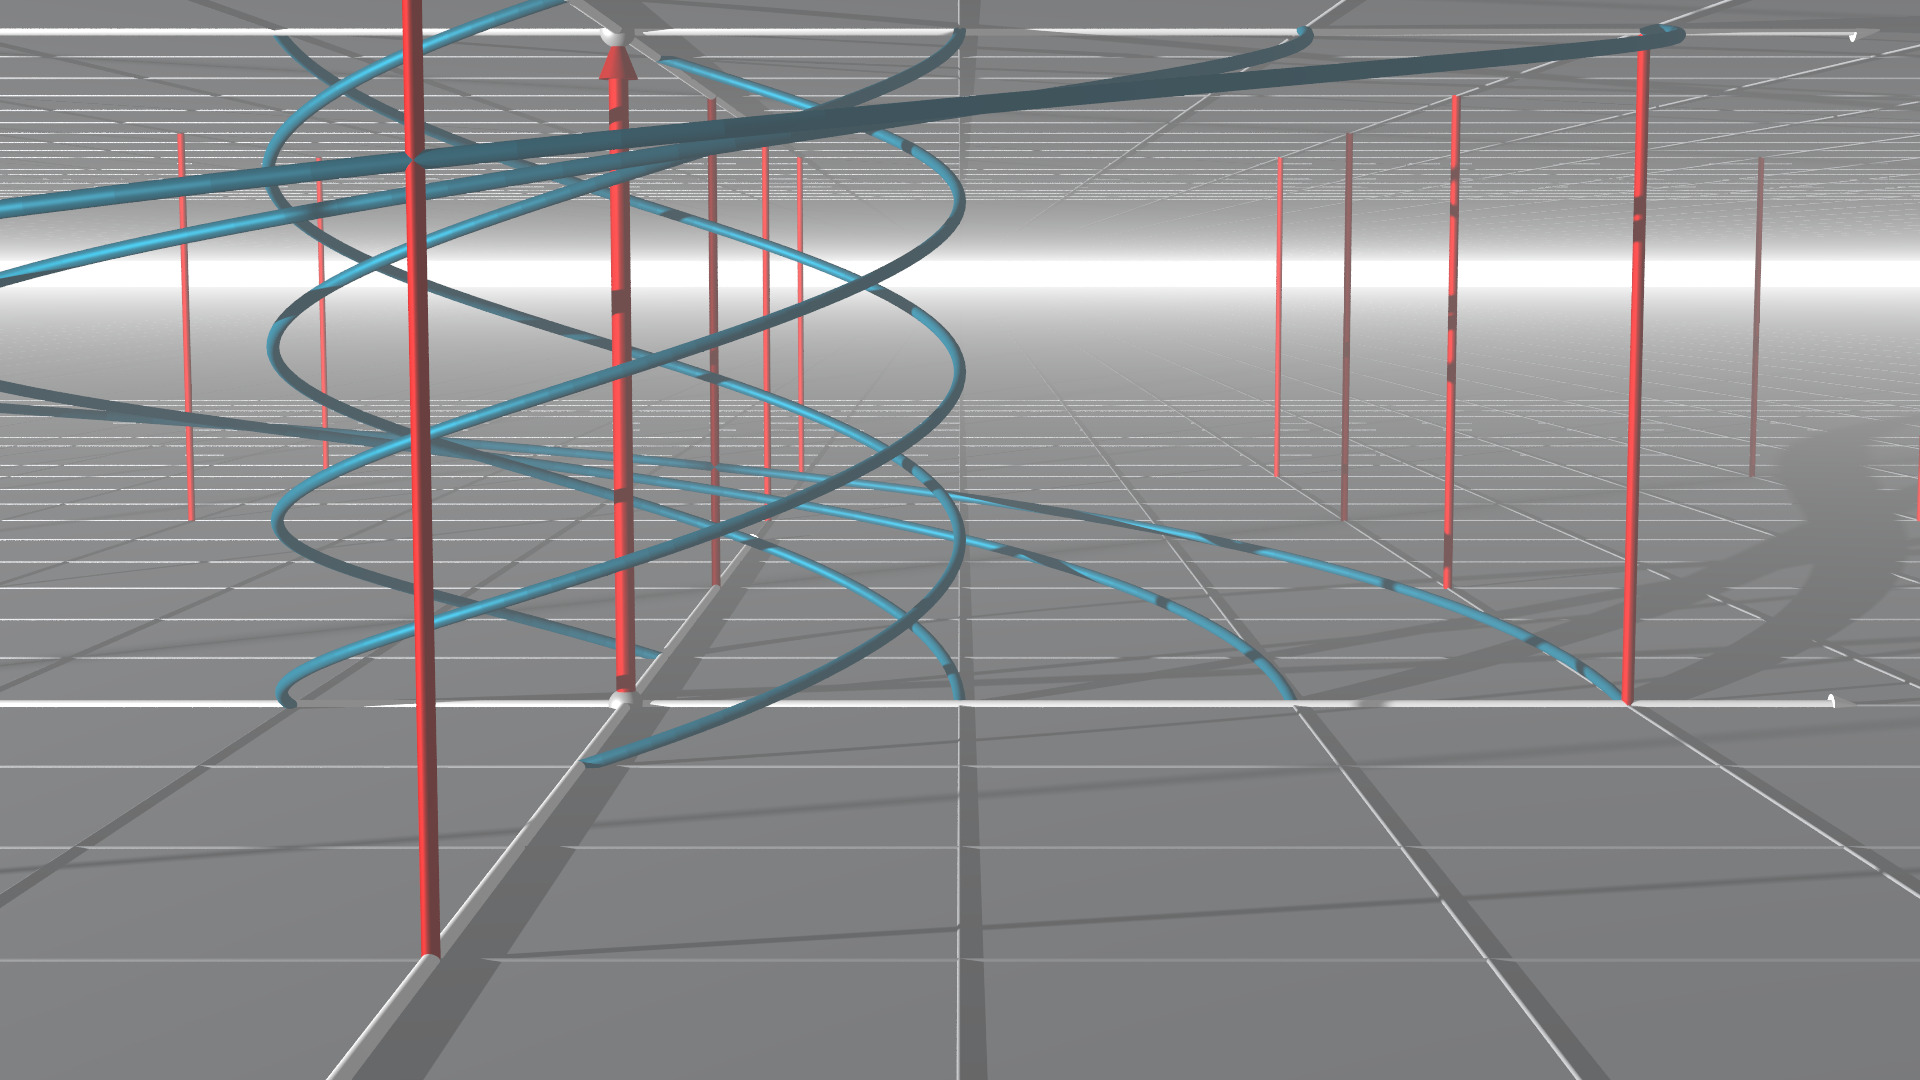
\includegraphics[width=14cm]{so2r2.jpg}};

% Gitter
\ifthenelse{\boolean{showgrid}}{
\draw[step=0.1,line width=0.1pt] (-\breite,-\hoehe) grid (\breite, \hoehe);
\draw[step=0.5,line width=0.4pt] (-\breite,-\hoehe) grid (\breite, \hoehe);
\draw                            (-\breite,-\hoehe) grid (\breite, \hoehe);
\fill (0,0) circle[radius=0.05];
}{}

\node at (6.4166,-1.225) [above] {$v_1$};
\node at (-1.225,0.058) {$v_2$};

%\draw[<->] (-2.3,-1.05) -- (-2.34,3.18);
%\node at (-2.3,1.3) [left] {$2\pi$};

\node at (-2.45,3.5) [left] {$\alpha$};
\node at (-2.68,-1.05) {$e$};

\end{tikzpicture}

\end{document}

